%%%%%%%%%%%%%%%%%%%%%%%%%%%%%%%%%%%%%%%%%
% Short Sectioned Assignment LaTeX Template Version 1.0 (5/5/12)
% This template has been downloaded from: http://www.LaTeXTemplates.com
% Original author:  Frits Wenneker (http://www.howtotex.com)
% License: CC BY-NC-SA 3.0 (http://creativecommons.org/licenses/by-nc-sa/3.0/)
%%%%%%%%%%%%%%%%%%%%%%%%%%%%%%%%%%%%%%%%%

% \documentclass[paper=a4, fontsize=11pt]{scrartcl} % A4 paper and 11pt font size
\documentclass[11pt, a4paper]{book}
\usepackage[T1]{fontenc} % Use 8-bit encoding that has 256 glyphs
\usepackage[utf8]{inputenc}
\usepackage{fourier} % Use the Adobe Utopia font for the document - comment this line to return to the LaTeX default
\usepackage{listings} % para insertar código con formato similar al editor
\usepackage[spanish, es-tabla]{babel} % Selecciona el español para palabras introducidas automáticamente, p.ej. "septiembre" en la fecha y especifica que se use la palabra Tabla en vez de Cuadro
\usepackage{url} % ,href} %para incluir URLs e hipervínculos dentro del texto (aunque hay que instalar href)
\usepackage{graphics,graphicx, float} %para incluir imágenes y colocarlas
\usepackage[gen]{eurosym} %para incluir el símbolo del euro
\usepackage{cite} %para incluir citas del archivo <nombre>.bib
\usepackage{enumerate}
\usepackage{hyperref}
\usepackage{graphicx}
\usepackage{tabularx}
\usepackage{booktabs}
\usepackage{appendix}

\usepackage[table,xcdraw]{xcolor}
\hypersetup{
	colorlinks=true,	% false: boxed links; true: colored links
	linkcolor=black,	% color of internal links
	urlcolor=cyan		% color of external links
}
\renewcommand{\familydefault}{\sfdefault}
\usepackage{fancyhdr} % Custom headers and footers
\pagestyle{fancyplain} % Makes all pages in the document conform to the custom headers and footers
\fancyhead[L]{} % Empty left header
\fancyhead[C]{} % Empty center header
\fancyhead[R]{Alejandro Menor Molinero} % My name
\fancyfoot[L]{} % Empty left footer
\fancyfoot[C]{} % Empty center footer
\fancyfoot[R]{\thepage} % Page numbering for right footer
%\renewcommand{\headrulewidth}{0pt} % Remove header underlines
\renewcommand{\footrulewidth}{0pt} % Remove footer underlines
\setlength{\headheight}{13.6pt} % Customize the height of the header

\usepackage{titlesec, blindtext, color}
\definecolor{gray75}{gray}{0.75}
\newcommand{\hsp}{\hspace{20pt}}
\titleformat{\chapter}[hang]{\Huge\bfseries}{\thechapter\hsp\textcolor{gray75}{|}\hsp}{0pt}{\Huge\bfseries}
\setcounter{secnumdepth}{4}
\usepackage[Lenny]{fncychap}
\graphicspath{ {./figuras/} } 


\begin{document}

	% Plantilla portada UGR
	\begin{titlepage}
\newlength{\centeroffset}
\setlength{\centeroffset}{-0.5\oddsidemargin}
\addtolength{\centeroffset}{0.5\evensidemargin}
\thispagestyle{empty}

\noindent\hspace*{\centeroffset}\begin{minipage}{\textwidth}

\centering

\includegraphics[width=0.9\textwidth]{logos/logo_ugr.jpg}\\[1.4cm]

\textsc{ \Large TRABAJO FIN DE GRADO\\[0.2cm]}
\textsc{ GRADO EN INGENIERIA INFORMATICA}\\[1cm]

{\Huge\bfseries Título \\}
\noindent\rule[-1ex]{\textwidth}{3pt}\\[3.5ex]
{\large\bfseries Subtítulo }
\end{minipage}

\vspace{2.5cm}
\noindent\hspace*{\centeroffset}
\begin{minipage}{\textwidth}
\centering

\textbf{Autor}\\ {Estudiante}\\[2.5ex]
\textbf{Director}\\ {Tutor(a)(es)}\\[2cm]

\includegraphics[width=0.3\textwidth]{logos/etsiit_logo.png}\\[0.1cm]
\textsc{Escuela Técnica Superior de Ingenierías Informática y de Telecomunicación}\\
\textsc{---}\\
Granada, Junio de 201x
\end{minipage}
\end{titlepage}


	% Plantilla prefacio UGR
	\thispagestyle{empty}

\begin{center}
{\large\bfseries Héroes \\ Geolocalización para ayuda en emergencias }\\
\end{center}
\begin{center}
Alejandro Menor Molinero\\
\end{center}

%\vspace{0.7cm}

\vspace{0.5cm}

\noindent{\textbf{Resumen}\\

La inseguridad en la vía pública, especialmente de las grandes ciudades, es un problema que muchas personas, sobre todo las mujeres, sufren cada día.
En mayor o menos medida nos podemos sentir vulnerables en la calle y nos gustaría estar acompañados. Héroes es una aplicación que permite conectar con personas
cercanas dispuestas a ayudar en muy poco tiempo. \\ \\
Para esto se ha implementado un servicio de geolocalización escalable con \mbox{NodeJS}, utilizando como infraestructura Redis y MongoDB, además de una aplicación
móvil con Flutter. El sistema permite alertar a personas cercanas, permitiéndolas seguir en tiempo real la ubicación de la víctima.
	

\cleardoublepage

\begin{center}
{\large\bfseries Héroes \\ Aid through geolocalization in emergencies}\\
\end{center}
\begin{center}
Alejandro Menor Molinero\\
\end{center}
\vspace{0.5cm}

\noindent{\textbf{Abstract}\\ \\
Insecurity in the streets, specially in big cities, it's a problem that many people, especially women, suffer every day.
We can feel vulnerable outside and we'd rather have company. Héroes is an app that allows us to connect with people nearby willing to help. \\ \\
To make this possible, an escalable geolocalization service has been implemented with NodeJS, using MongoDB and Redis as infraestructure, besides 
a mobile App with Flutter. The system sends an alert to nearby people, enabling them to follow the victim's location in real time.


\cleardoublepage

\thispagestyle{empty}

\noindent\rule[-1ex]{\textwidth}{2pt}\\[4.5ex]

D. \textbf{Juan Julián Merelo Guervós}, profesor del departamento de Arquitectura y Tecnología de Computadores.

\vspace{0.5cm}

\textbf{Informo:}

\vspace{0.5cm}

Que el presente trabajo, titulado \textit{\textbf{Héroes}},
ha sido realizado bajo mi supervisión por \textbf{Alejandro Menor Molinero}, y autorizo la defensa de dicho trabajo ante el tribunal
que corresponda.

\vspace{0.5cm}

Y para que conste, expiden y firman el presente informe en Granada a Julio de 2021.

\vspace{1cm}

\textbf{El/la director(a)/es: }

\vspace{5cm}

\noindent \textbf{Juan Julián Merelo Guervós}







	% Índice de contenidos
	\newpage
	\tableofcontents

	% Índice de imágenes y tablas
	\newpage
	\listoffigures


	\chapter{Introducción}

Este proyecto es software libre, y está liberado con la licencia \cite{gplv3}.

\section{El problema}
En pleno 2021, en España, la calle no es siempre un lugar seguro. Dependiendo de la zona por la que te muevas, la hora o tu género
hay más o menos probabilidades de que te lleves, en el mejor de los casos, un susto.

Los últimos estudios, como el de RACC y Zurich \cite{racc-zurich}, sacan conclusiones muy preocupantes, por ejemplo: 
\begin{itemize}
  \item El 45\% de las mujeres encuestadas declara que ha sido víctima de acoso de noche en la vía pública yendo a pie.
  \item El 68\% y 37\% de mujeres y hombres respectivamente ha cambiado alguna vez de modo de transporte por motivos de seguridad personal.
\end{itemize}

\section{Estado del arte}\label{sec:art}
Durante los últimos años, han ido emergiendo distintas aplicaciones que tratan de paliar esta inseguridad que podemos clasificar en dos grupos:
\begin{enumerate}
\item \textbf{Botón del pánico a la policía:} En caso de estar en una situación complicada, podemos avisar a la policía sin necesidad de llamar. La más famosa es \textbf{AlertCops} que cuenta con el respaldo del ministerio del interior.
\item \textbf{Botón del pánico a un grupo de contactos:} Con una activación similar a el grupo anterior, el aviso esta vez se hace a una serie de personas cercanas. En muchos casos, estas serán capaces de saber donde estás, escuchar y ver lo que pasa a partir de ese momento. Algún ejemplo: \textbf{bSafe}, \textbf{When and Where} o \textbf{Companion}.
Otra ''implementación'', es la creación de grupos de mensajería masivos de estudiantes para pedir ayuda si se sienten inseguras.
\end{enumerate}

\section{Inconvenientes}
Pese a la cantidad de alternativas y a la alta calidad de muchas de ellas, no han conseguido tener el impacto que esperaban.
\begin{enumerate}
  \item La policía o los contactos están, en muchos casos, lejos de ti y la ayuda tiene que ser inmediata.
  \item A veces el peligro no es explícito y pedir auxilio es excesivo, por ejemplo: sospechas que alguien te está siguiendo.
\end{enumerate}

\section{Análisis del problema}
Queremos reducir al máximo la inseguridad de todas las personas en la vía pública.

Podemos identificar tres niveles dentro del problema:
\begin{enumerate}
  \item \textbf{Sospecha, ligera inseguridad:} No lo sabes con certeza, pero algo te pone alerta, podrías estar en peligro y te gustaría estar acompañado.
  \item \textbf{Miedo:} Estás en una situación totalmente incómoda, no sabes si va a llegar a más, pero necesitas compañía.
  \item \textbf{Pánico:} Es necesaria una ayuda inmediata y sería pertinente avisar a los cuerpos de seguridad.
\end{enumerate}

Para los dos primeros, que a su vez son las más comunes, no hay propuestas.

\section{Objetivos generales}\label{sec:obj}
\begin{enumerate}
  \item La solución tiene que cubrir la funcionalidad de los botones del pánico existentes, analizados en la sección \ref{sec:art}.
  Dar la posibilidad de: 
  \begin{itemize}
    \item Avisar a la policía con un botón en una situación de auxilio.
    \item Avisar a un grupo de contactos de confianza con un botón, compartiendo ubicación, audio y video.
  \end{itemize}
  Configurable por el usuario.
  \item Deberá recoger toda la información relevante del entorno que pueda servir para esclarecer los hechos.
  \item La solución tiene que ser efectiva para los primeros niveles de inseguridad descritos anteriormente.
  \begin{itemize}
    \item Dar la posibilidad de que alguien que esté cerca te acompañe si lo necesitas.
    \item Dar la posiblidad de prestar esa ayuda.
  \end{itemize}
En este trabajo, vamos a plantear y a implementar una solución para este objetivo.
\end{enumerate}



	\chapter{Planificación}

Antes de hablar de detalles de implementación, tenemos que pensar en la metodologia y el control de calidad de la solución a construir.

\section{Metodología}

Necesito una metodología \textbf{que ponga al usuario en el centro} y permita una \textbf{retroalimentación rápida.} \\
\textbf{La metodología ágil} evita la documentación intensiva de requisitos y más diagramas de los necesarios, en favor de la iteración y la adaptación a requisitos cambiantes.\\

Otro principio de esta filosofía son las aportaciones frecuentes de código que aporten valor al usuario. Para esto, 
necesitamos organizar la funcionalidad en bloques y asegurarnos de que los cambios en el código siempre surgen
de una necesidad del usuario.
\begin{enumerate}
	\item Los conceptos que expongo más abajo ayudan a esa organización.
	\item Es importante que \textbf{los commits pueden referencien a estas tareas.} Así podemos
saber no solo quién ha escrito una línea de código sino también \textbf{por qué}, que siempre deberá responderse con una historia de usuario (\ref{subsec:hu}) o un issue (\ref{subsec:issue}).
\end{enumerate}

\begin{figure}[H]
\centering	
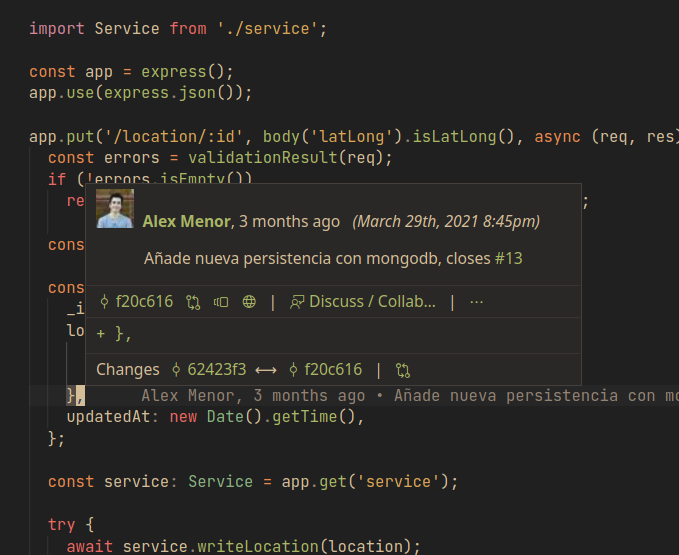
\includegraphics[scale=0.6]{git.png}
\end{figure}

Además, aplicando técnicas de design thinking, se ha hecho un análisis de "Personas" \cite{personas}. Ver anexo \ref{anexo}.

\subsection{Control de versiones}
Como sistema de control de versiones utilizo Git y como repositorio remoto GitHub \cite{repo}. Además, como veremos en la sección \ref{sec:inc} y \ref{sec:cal} GitHub
también nos permite implementar los flujos de integración continua y organizar las tareas.

\subsection{Iniciativas}\label{sec:inc}
\textbf{Son grandes grupos de funcionalidad, independientes entre sí, que sirven para atacar el problema.}
Acorde a lo explicado en la sección \ref{sec:obj}, he propuesto las tres iniciativas y las he 
reflejado como proyectos dentro del repositorio de GitHub.
\begin{figure}[H]
\centering	
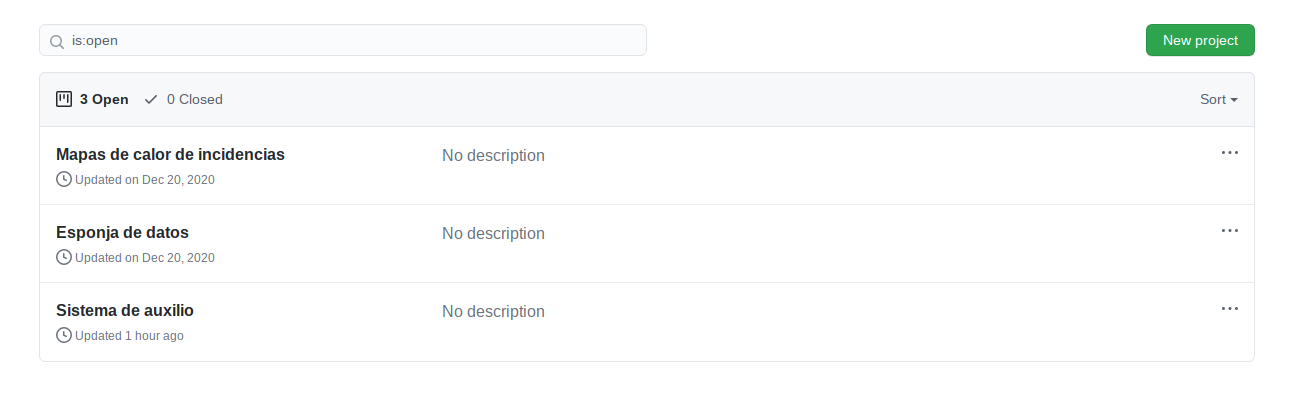
\includegraphics[scale=0.4]{iniciativas.png}
\end{figure}

\subsection{Épica}
Una iniciativa está formada por varias épicas. \textbf{Una épica por si sola no es una solución al problema}, pero todas las épicas de una iniciativa contribuyen a la solución.
Por ejemplo, para la iniciativa del sistema de auxilio, tenemos 
como épicas el frontend y el backend. Se reflejan en GitHub como milestones.
\begin{figure}[H]
	\centering
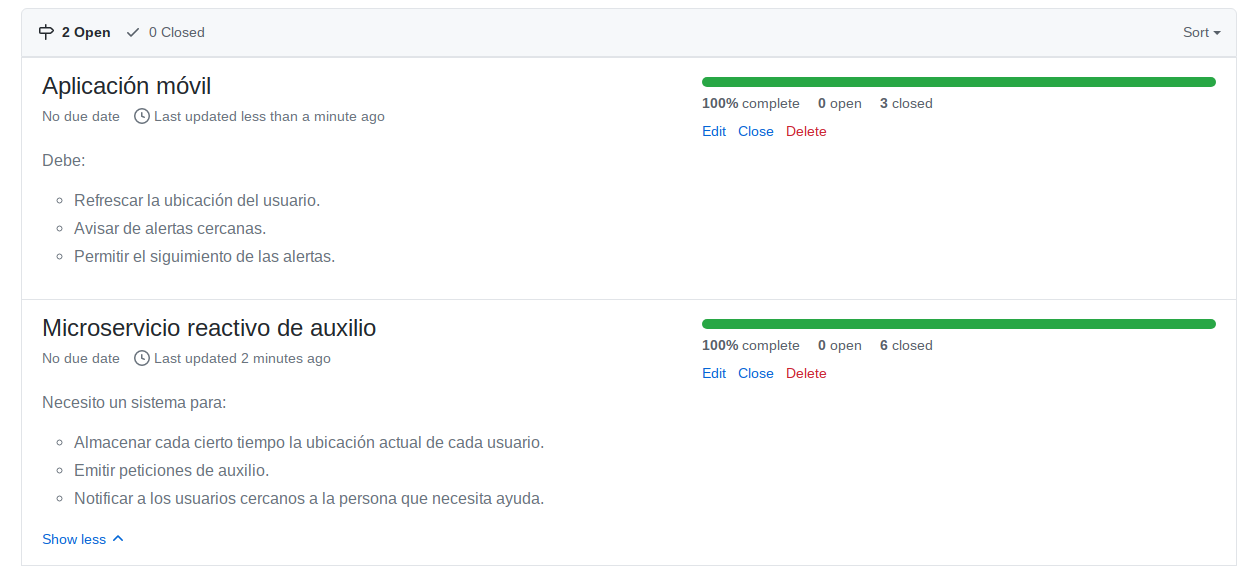
\includegraphics[scale=0.4]{milestones.png}
\end{figure}


\subsection{Historia de usuario}\label{subsec:hu}
Una épica a su vez está formada por varias historias de usuario que definen \textbf{una funcionalidad que el usuario espera en una solución}, de la forma:\\ \textit{Como [rol] quiero [funcionalidad] para [razón].}\\

A la hora de implementar una historia de usuario, esta se puede definir con requisitos más detallados.

\begin{figure}[H]
	\centering	
	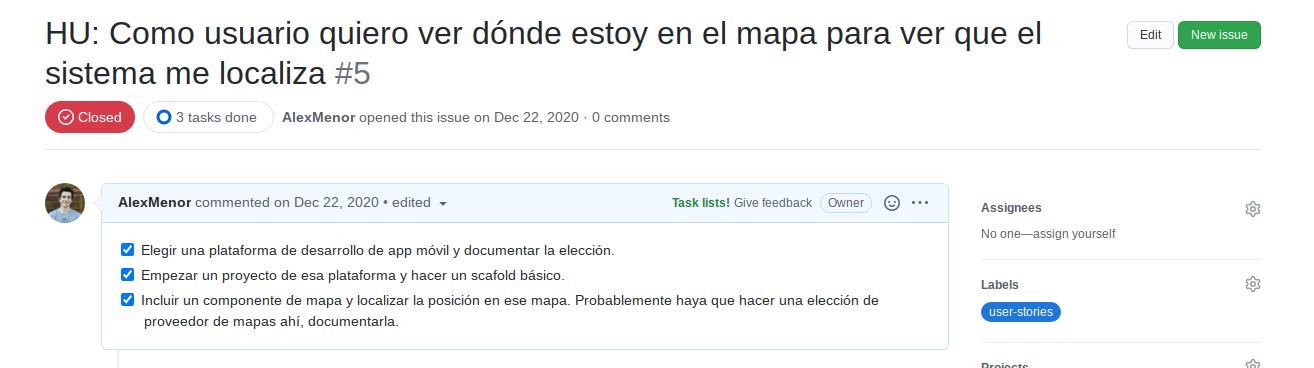
\includegraphics[scale=0.4]{hu.png}
	\end{figure}

\subsection{Issues}\label{subsec:issue}
\textbf{Cuando no se obtiene el comportamiento esperado}, podemos abrir un issue que se cerrará con un commit que lo solucione e idealmente un test que lo detecte.

\begin{figure}[H]
	\centering	
	
\includegraphics[scale=0.4]{issue.png}
	\end{figure}

	También pueden ser issues tareas que faciliten el mantenimiento del código.

\begin{figure}[H]
	\centering	
	
\includegraphics[scale=0.4]{issue2.png}
	\end{figure}


\section{Control de calidad}\label{sec:cal}

Para asegurar la calidad del proyecto necesitamos utilizar \textbf{integración continua con tests y análisis estático del código} por medio de linters (ver sección \ref{sec:tools}).


Cada vez que se hace un commit, se ejecutan todos estos procesos automáticamente.

La presencia de tests, de la que hablo con más detalle en la sección \ref{sec:tests}, nos permite, entre otras cosas, refactorizar con más 
tranquilidad. \\

Para cubrir la parte de integración continua he utilizado Github Actions,  configurando en formato \textit{yaml} todos los flujos.\\
La implementación continua de los tests y linters dependen del lenguaje y otros detalles de implementación, por tanto
son distintos para cada entorno.
\begin{figure}[H]
	\centering	
	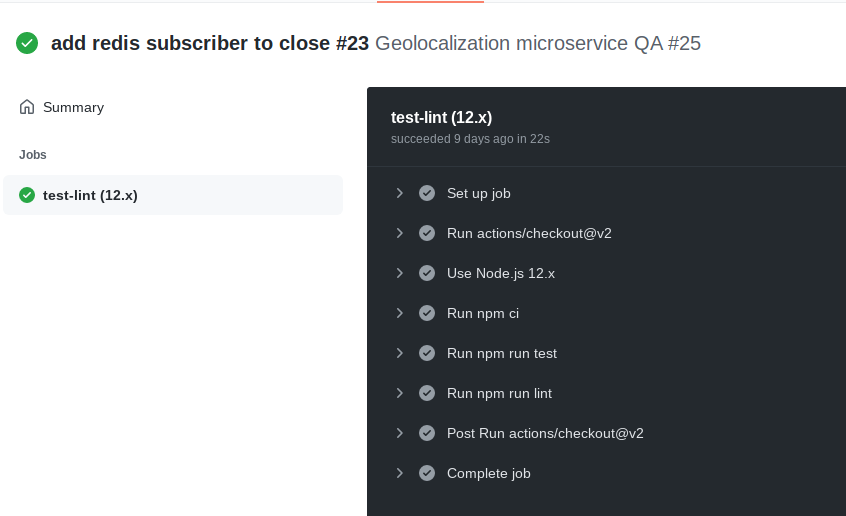
\includegraphics[scale=0.4]{ci.png}
	\end{figure}





	\chapter{Implementación}
En primer lugar tenemos que decidir entre un sistema \textit{peer to peer} \cite{p2p} o uno con arquitectura de cliente-servidor \cite{client-server}.
Creo que la decisión más apropiada es la segunda, pues nos permite más control y simplifica mucho el diseño. \\\\
Tenemos dos partes bien diferenciadas.
\begin{itemize}
	\item  \textbf{La parte del cliente,} que se encargaría de actualizar con cierta frecuencia
la ubicación de cada usuario, recibir un aviso cuando haya alguien cercano que necesite ayuda y permitir realizar el seguimiento de una alerta.
\item Por otro lado, \textbf{la parte del servidor} recibe tanto las actualizaciones en cuanto a ubicación como 
los avisos de alerta. Se encarga por tanto de hacer los cálculos para saber a quién avisar y hacerlo. \\
Una vez la víctima y la persona que se presta a ayudar están conectadas, el servidor debe mantener
al cliente informado sobre la localización de la víctima y el estado de la alerta. \\
\end{itemize}

\section{Backend}
La mayoría de la lógica de la aplicación está en este componente, por lo que descartamos un BaaS \cite{baas}, que sería más apropiado en el caso de un cliente 
muy rico y un backend que se encargue solamente de la autenticación y la persistencia. \\ \\

En esta sección voy a hablar de \textbf{la implementación de este microservicio de geolocalización}.
\subsection{Lenguaje de programación}
Necesito un lenguaje que me permita modelar bien el dominio, tenga un buen ecosistema y proporcione una buena experiencia de desarrollo, evitando lenguajes demasiado estrictos y ''verbosos''.
He decidido usar \textbf{Typescript} \cite{typescript}, que es un lenguaje de tipado gradual que transpila \cite{transpiler} a Javascript \cite{javascript}.
Como ventajas sobre Javascript:
\begin{itemize}
	\item Mejor \textit{developer experience}, sobre todo gracias al autocompletado.
	\item \textbf{Detección de errores precoz gracias a los tipos.}
\end{itemize}
Es cierto, sin embargo, que añade más complejidad en el setup de desarrollo (y también en el de despliegue) del que hablo en la sección \ref{sec:dev}. \\ \\
\textbf{Considero que es un \textit{sweet spot} entre la excesiva libertad en Javascript y la rigidez de lenguajes tipados estrictos como Java o C\#.} \\ \\

\textbf{Como runtime he elegido Node \cite{nodejs}.} Utiliza una sola hebra con E/S no bloqueante, lo cuál se ajusta bien al tipo 
de peticiones que se atienden en este backend (sin cómputos extensos).  \\ \\
Como alternativa, podría haber elegido Deno \cite{deno}, pero no tiene un ecosistema aún tan desarrollado.
Como gestor de paquetes, he utilizado NPM \cite{npm}.

\subsection{Framework}
\textbf{La API será, por simplicidad, REST \cite{rest}.} Necesitamos un framework para implementar esta interfaz. \\\\
Hay muchas alternativas en este ecosistema, como: Koa, Fastify o Hapi. Las diferencias entre ellos tienen que ver sobre todo con rendimiento, documentación y la interfaz (de cara al desarrollador). \\
De todas formas, gracias a la arquitectura limpia (\ref{sec:clean}), el esfuerzo
para cambiar a otro sería mínimo. \\
\textbf{He decido usar Express \cite{express}, que es un framework \textit{unopinionated} muy consolidado.} 


\subsection{Setup de desarrollo}\label{sec:dev}

He invertido tiempo en tener \textbf{un entorno de desarrollo replicable por cualquiera que esté interesado en trabajar en este proyecto.}
Por eso, he usado Docker y Docker Compose \cite{docker}. He creado un \textit{Dockerfile} que encapsula el microservicio. 
\\ Por último, en Docker Compose arranco y comunico el microservicio y los otros procesos (base de datos y pub/sub). \\ \\
\textbf{Las instrucciones para iniciar un entorno de desarrollo son las siguientes:}

\begin{enumerate}
	\item En el archivo \textit{.env.template} están recogidas las variables de entorno que hacen falta para configurar este microservicio.
Podemos simplemente copiar este archivo a otro de nombre \textit{.env} y \textit{dotenv} se encargará de usarlas (ver sección \ref{sec:config}).
\item También necesitamos un archivo \textit{serviceAccountKey.json} que se puede obtener en Firebase Cloud Messaging \cite{firebase} y que hay que situar en este directorio. 
(En el .gitignore está declarado este archivo porque contiene claves privadas.)
\item Una vez hecho esto, simplemente ejecutamos: \textbf{\textit{docker-compose up}}.
\end{enumerate}

\subsection{Base de datos}

Necesito una base de datos que \textbf{soporte un gran volumen de operaciones (especialmente actualizaciones) y permita consultas basadas en localizaciones geográficas.} \\ \\
\textbf{En el CAP Theorem \cite{cap} necesito la A (de availability) y la P (de partition tolerance), sacrificando la consistencia.}
\\
En esta base de datos se almacenará de manera periódica la ubicación de cada uno de los usuarios con el fin de una consulta posterior, que nos permita saber qué usuarios
están cerca de una persona que necesita ayuda. Por ello, es más que suficiente la \textbf{consistencia eventual.}

\subsubsection{Opciones}

\begin{itemize}
	\item \textbf{MongoDB tiene buen soporte para \textit{geo-queries}} \cite{mongo}, de hecho vienen ya instaladas, sin embargo, \textbf{prioriza la consistencia antes que la disponibilidad \cite{mongo-cap}.} 
\item \textbf{PostgreSQL}, con PostGIS \cite{postgis}, \textbf{también soporta bien este tipo de consultas, pero prioriza la consistencia a la tolerancia a la partición.} 
\item \textbf{CouchDB, Dynamo y Cassandra son sistemas con alta disponibilidad y tolerancia a la partición.} CouchDB es la mejor opción porque Dynamo es privativa y Cassandra es más adecuada para aplicaciones con más
escrituras que actualizaciones \cite{cassandra}. 
\end{itemize}



Tras probar CouchDB me di cuenta de que \textbf{el soporte para queries de geolocalización} no es bueno \cite{couchdb}.

\textbf{Acabe optando por MongoDB} que sí tiene buen soporte.

Además, puedo habilitar la escritura en replicas para cambiar la consistencia estricta por consistencia eventual y tener más disponibilidad. 

\subsubsection{Configuración de MongoDB}

En el archivo \textit{mongo-init.js} se crea el usuario que se va a utilizar desde el microservicio y el índice "2dsphere". 
En Docker Compose lo monto como volumen para que lo pueda ejecutar en tiempo de inicialización la instancia que se declara ahí.

\subsection{Arquitectura limpia}\label{sec:clean}

He tratado de mantener en todo momento \textbf{el dominio desacoplado de los detalles de infraestructura, de la interfaz de usuario y de cualquier framework.}
\begin{figure}[H]
	\centering	
	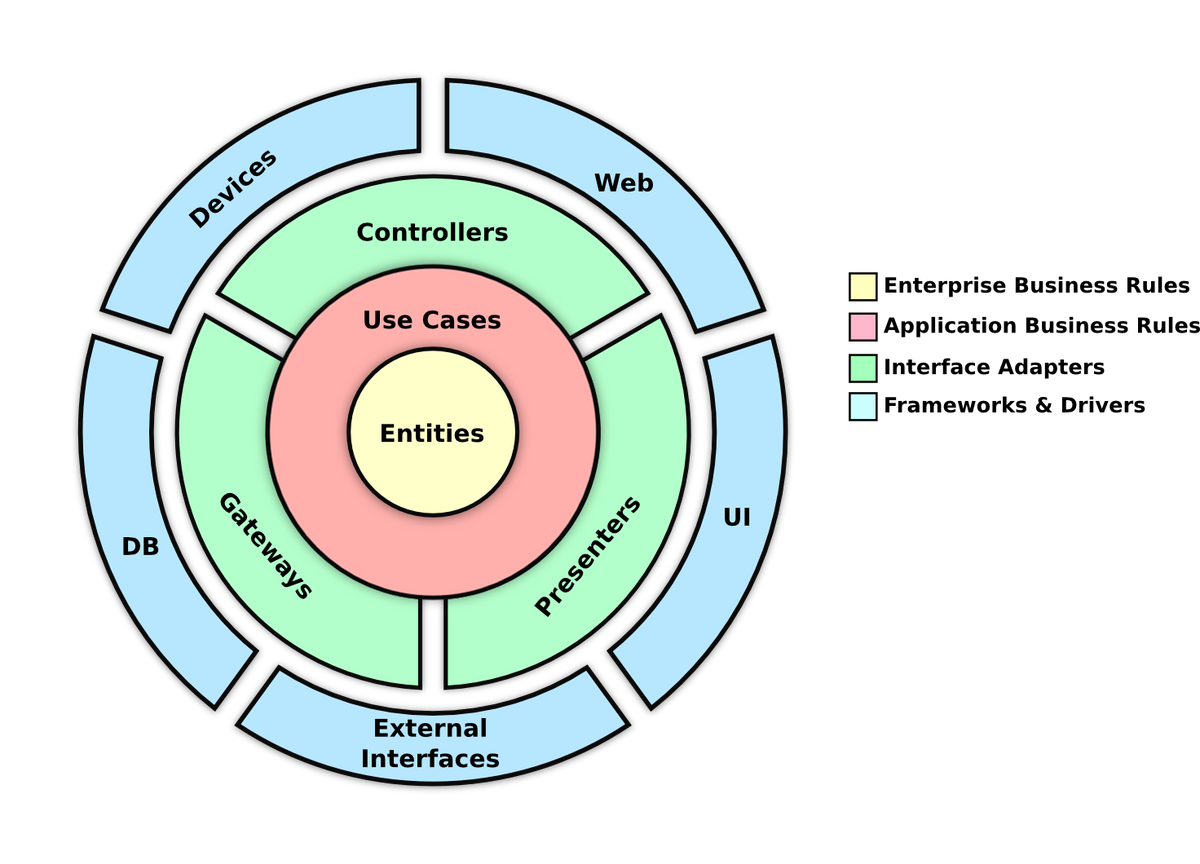
\includegraphics[scale=0.3]{clean_arc.png}
	\caption{Esquema de arquitectura limpia \cite{clean-arch}}
	\end{figure}

\textbf{Tenemos tres capas bien diferenciadas:}


\subsubsection{Aplicación}
En este caso es una \textbf{API REST implementada con Express.} Toma peticiones HTTP, extrae la información, la valida, usa métodos expuestos del dominio y devuelve información.
Aparte, también hay un endpoint \textbf{websocket} que explico en la subsección \ref{subsec:websocket}. \\
Considero importante separar bien esta capa del servicio de dominio que consume. Con esto, sería sencillo dejar de usar 
REST para utilizar \textit{SOAP} o \textit{GraphQL}, por ejemplo. \textbf{Incluso podríamos utilizar otro framework con esfuerzo mínimo.}

\subsubsection{Dominio}
\textbf{Tipos y casos de uso que pertenecen exclusivamente al dominio.}
Cuando estos casos de uso necesitan utilizar un servicio de infraestructura como el de persistencia, por ejemplo,
\textbf{se depende exclusivamente de una interfaz que describe esa función y se inyecta en tiempo de ejecución un servicio que la implemente (inyección de dependencias).}
\\Evitamos diseñar el sistema alrededor de su infraestructura, por ejemplo, una determinada base de datos, \textbf{en favor de hacerlo alrededor del dominio.}
\begin{figure}[H]
	\centering	
	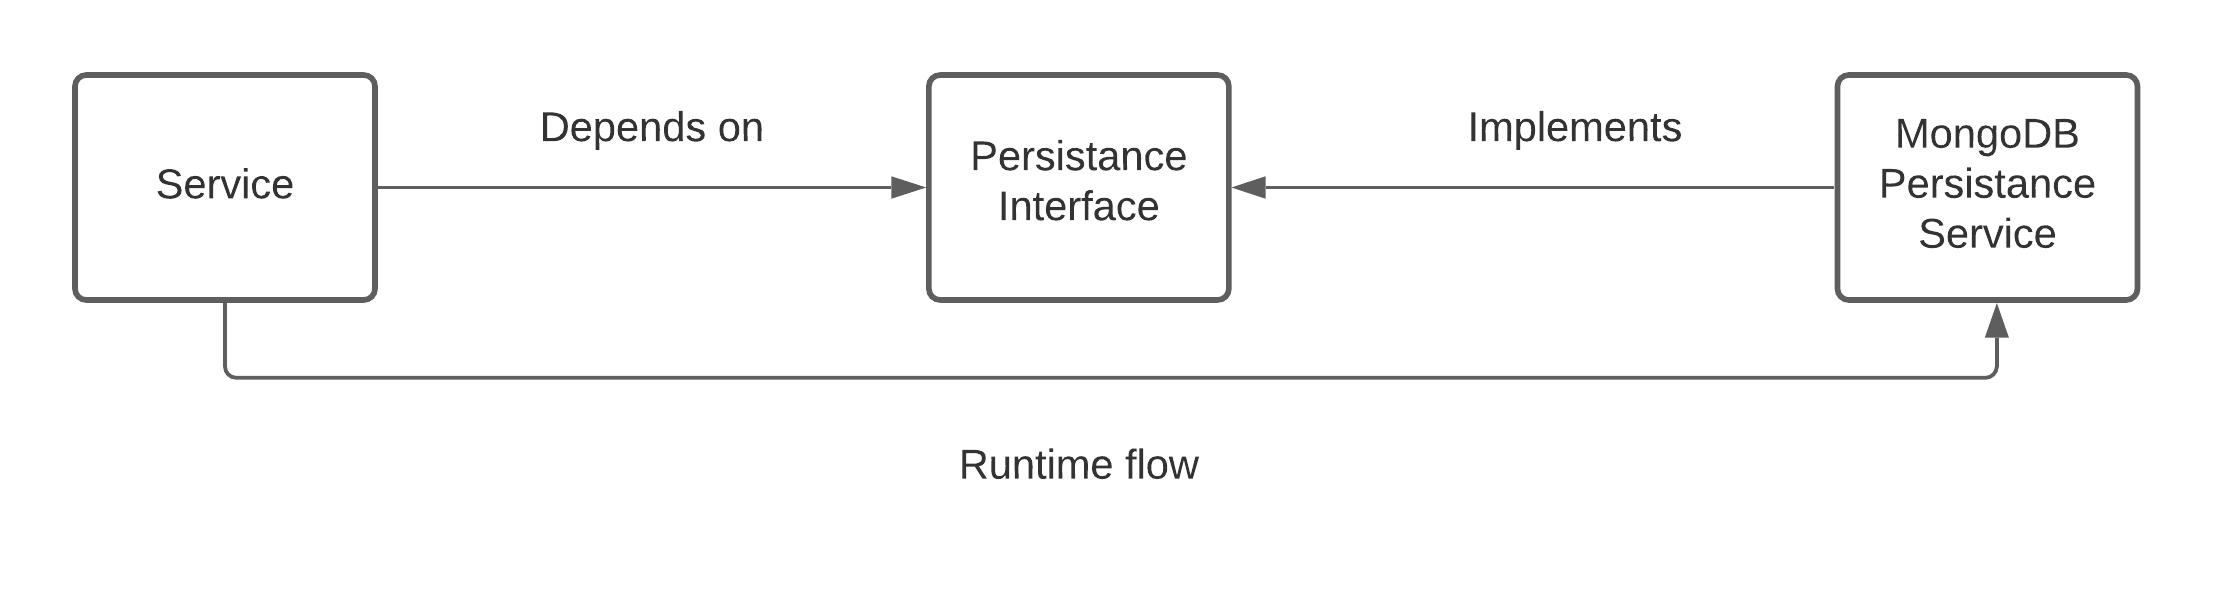
\includegraphics[scale=0.7]{di.png}
	\caption{Inyección de dependencias}
	\end{figure}

Asimismo, \textbf{esta separación incrementa mucho la testeabilidad del microservicio,} porque las únicas dependencias
que puede tener esta capa forman parte del lenguaje de programación. Podemos usar \textit{mocks} para implementar
las interfaces de infraestructura y probar todas las posibles respuestas de estos servicios. \\ \\
Por último, he comentado concienzuadamente las interfaces con \textbf{JSDoc} \cite{jsdoc} para facilitar la implementación de otros servicios.
\begin{figure}[H]
	\centering	
	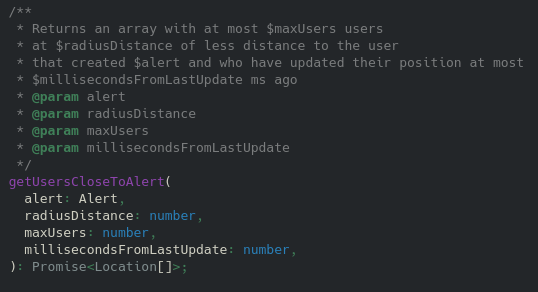
\includegraphics[scale=0.9]{jsdoc.png}
	\end{figure}

\subsubsection{Infraestructura} 
Son servicios que implementan las interfaces de las que acabo de hablar.
En este capa está la lógica para comunicarse con los distintos servicios: Bases de datos, mensajería, etc...
\begin{figure}[H]
	\centering	
	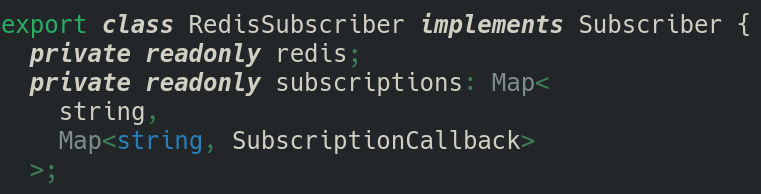
\includegraphics[scale=0.6]{imp.png}
	\end{figure}


\subsection{Operaciones}

Descripción en líneas generales de los tipos de peticiones que debe atender el backend:

\subsubsection{Crear/Actualizar ubicación}\label{op:ubi}
Toma unas coordenadas y un id de usuario y persiste en la base de datos.
Esta operación es indispensble para avisar a los usuarios cercanos a una emergencia y para 
actualizarlos sobre la posición de una víctima (publicando la ubicación actualizada en el pub/sub, sección \ref{sec:pubsub}).

\subsubsection{Crear alerta}
Verificando antes que el usuario no tiene ya otra alerta en curso, la persiste.
Busca todos los usuarios cercanos que hayan actualizado su ubicación recientemente y les avisa. Para hacer
esta consulta rápidamente, la operación \ref{op:ubi} indexa las ubicaciones.
Mientras siga en estado activo, se verifica que el usuario sigue actualizando su ubicación, de lo contrario la alerta pasa a estado inactivo.

\subsubsection{Escuchar alerta}\label{subsec:websocket}
Los usuarios a los que se ha avisado de la alerta pueden empezar a escuchar actualizaciones de la alerta,
ya sea porque el usuario que la creó cambia su posición o porque la alerta es ya inactiva. \\
Para esto:
\begin{enumerate}
	\item El cliente y el servidor mantienen un websocket abierto.
	\item Se subscribe a los cambios en la alerta o en la ubicación.
	\item Cuando estos cambios se producen, se emiten por el websocket al cliente.
	\item Si la alerta pasa a estado inactivo, el websocket se cierra y se desubscribe.
\end{enumerate}
\textbf{Utilizo websockets porque permite al servidor hacer "push" de información sin que el cliente tenga que hacer "polling".}
He considerado que podría utilizar otros protocolos como SSE (server sent events) y una implementación más peer to peer con WebRTC por ejemplo, conectando directamente los dispositivos interesados.

Es cierto que quitaría carga al servidor, pero también aumentaria la complejidad.

\subsubsection{Borrar alerta}
Se marca una alerta existente como inactiva. Si hay usuarios pendientes de esta alerta, se les avisa.


\subsection{Pub/Sub}\label{sec:pubsub}
\textbf{Al usar websockets}, teniendo en cuenta que queremos tener escalado horizontal en este servicio,
\textbf{necesitamos un sistema de publicación/subscripción.} \\
Puesto que va a tener una función muy específica, este sistema ha de ser fácil de escalar, configurar y usar.
RabbitMQ, Amazon SNS o Cloud Pub/Sub son algunas opciones. \\ \\
Sin embargo, \textbf{he elegido Redis \cite{redis}}, que cuenta con una interfaz más simple que RabbitMQ y es open source a diferencia de las otras dos opciones.\\ 
Como librería, ioredis, que es muy robusta y rápida.\\ \\

Para escalar, tendríamos que añadir más instancias del microservicio y potenciar el cluster de redis para la comunicación entre ellas.

\begin{figure}[H]
	\centering	
	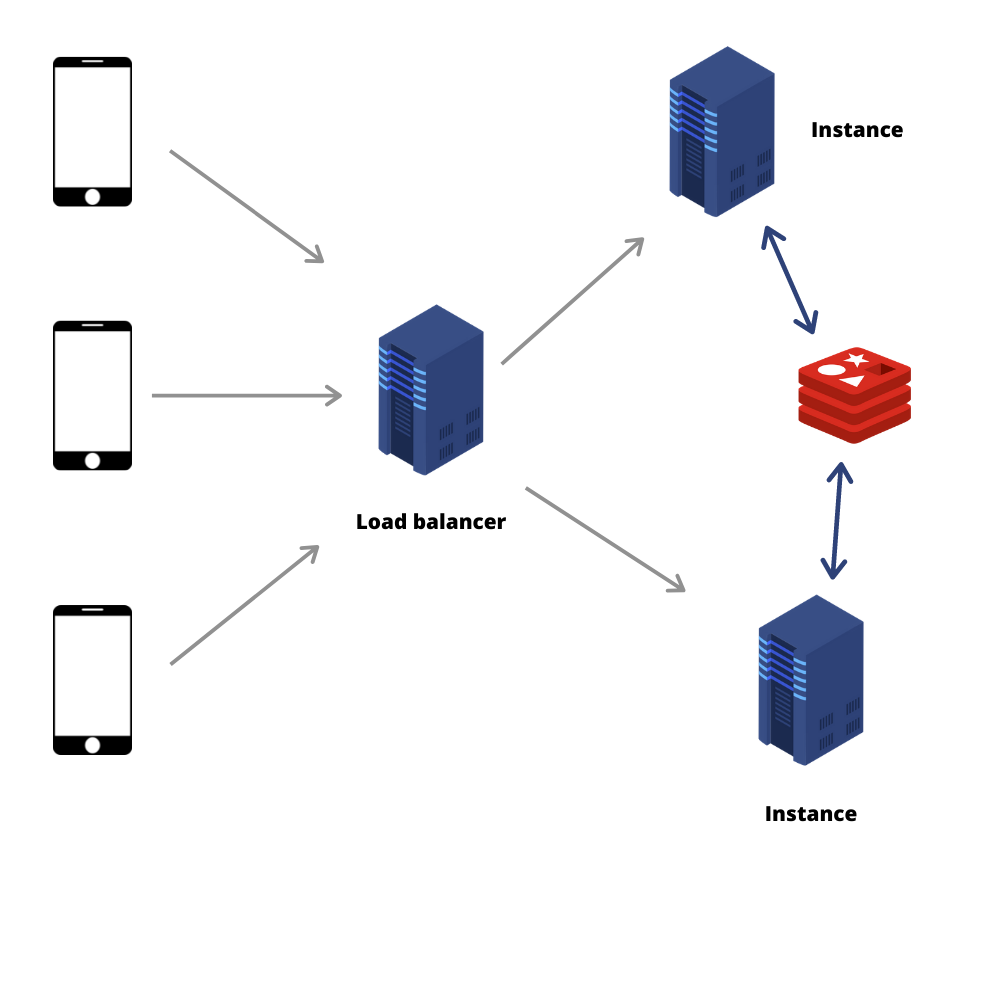
\includegraphics[scale=0.4]{pubsub.png}
	\end{figure}

\textbf{Por cada instancia del microservicio, tenemos dos conexiones a Redis:}
\subsubsection{Publisher}

Este servicio simplemente se conecta a Redis y \textbf{publica entidades en el momento en el que se modifican} (ubicaciones y alertas).
Publica al canal definido con el id de la entidad, esta misma serializada en JSON.

\subsubsection{Subscriber}
Este servicio es algo más sofisticado. \textbf{Mantiene en un Map los canales a los que está subscrito y 
para cada canal todas las subscripciones.} Estas mismas tienen un id para manejar la desubscripción (generado en tiempo de creación) y 
el callback que hay que ejecutar cuando llega una publicación para esa subscripción. 
\begin{figure}[H]
	\centering	
	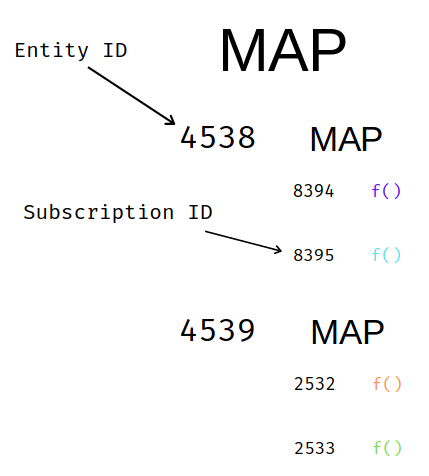
\includegraphics[scale=0.8]{map.png}
	\caption{Estructura de datos en Subscriber}
	\end{figure}
Cuando un websocket se cierra, las subscripciones asociadas desaparecen de esta estructura.
\subsection{Envío de notificaciones}\label{sec:fibpre}
\textbf{Para avisar a las personas cercanas de que alguien necesita ayuda, tenemos que tener la habilidad de enviar
notificaciones push.} Para esto he usado Firebase Cloud Messaging, del que hablo más en la sección \ref{sec:fib}.

\subsection{Tests}\label{sec:tests}
En este microservicio uso Jest y Supertest \cite{supertest} para \textbf{testear las capas de aplicación y dominio, con mocks de la capa de infraestructura.} \\ \\
Como próximos pasos, deberíamos implementar tests unitarios para la capa de dominio y especialmente la de infraestructura.
\begin{figure}[H]
	\centering	
	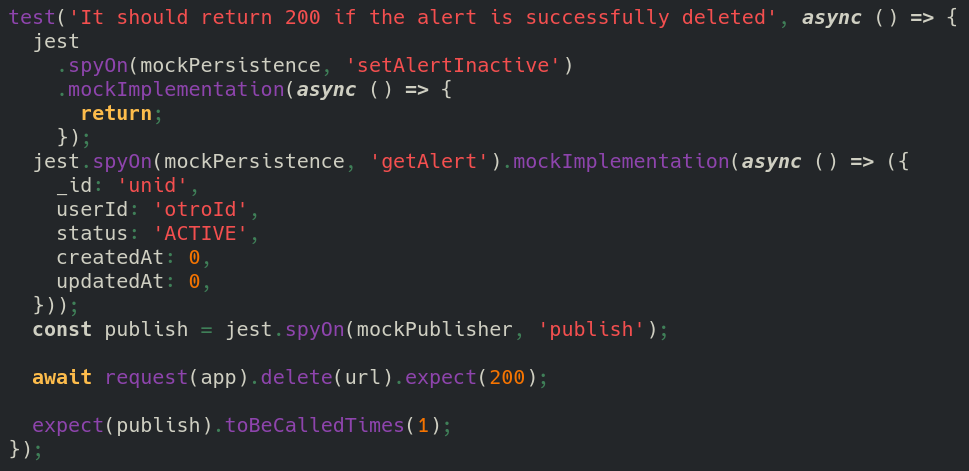
\includegraphics[scale=0.5]{test.png}
	\end{figure}

\subsection{Configuración}\label{sec:config}
\textbf{Las variables de configuración se definen mediante variables de entorno.} Para desarrollo uso \textit{dotenv}, 
que las carga de un archivo de configuración.
\begin{figure}[H]
	\centering	
	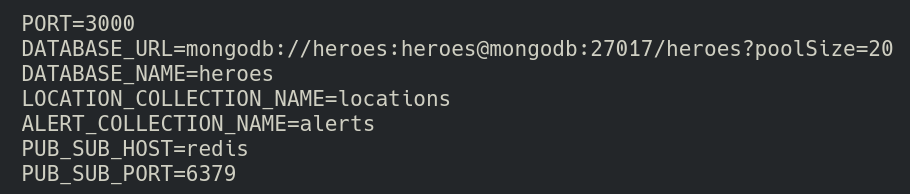
\includegraphics[scale=0.5]{env.png}
	\end{figure}

	Por otro lado, \textbf{los parámetros de configuración que tengan que ver con la lógica
	de negocio, los he declarado y documentado en el servicio de dominio.}

\begin{figure}[H]
	\centering	
	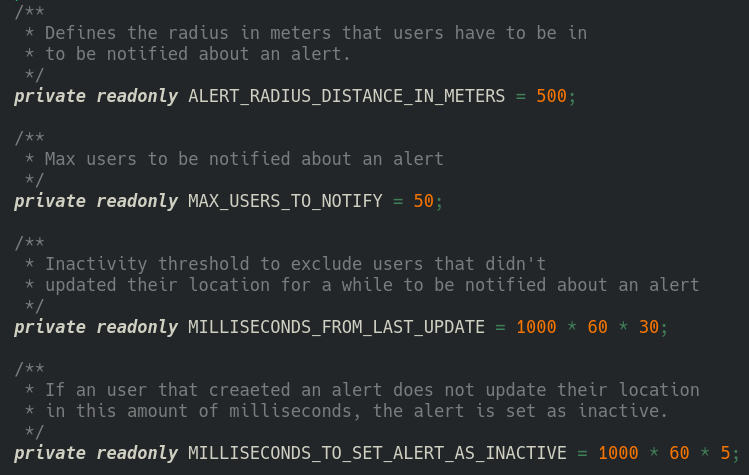
\includegraphics[scale=0.6]{conf.png}
	\end{figure}



\subsection{Otras herramientas}\label{sec:tools}
Otras herramientas que he utilizado en esta parte son:
\begin{itemize}
	\item \textbf{Express-validator} para validar los cuerpos de las peticiones HTTP
	\item \textbf{ESLint} para mantener las buenas prácticas.
	\item \textbf{Prettier} para el formateo del código.
	\item \textbf{Nodemon} para reiniciar el microservicio cada vez que hay cambios durante el desarrollo.
	\item \textbf{Concurrently} para ejecutar con un solo comando (\textit{npm run dev}) el watcher de Typescript y Nodemon.
\end{itemize}

\section{Frontend}
La segunda parte del sistema de auxilio es el cliente, \textbf{el código que se ejecuta en el dispositvo del usuario.}
\subsection{Elección de la tecnología}
Nunca hemos tenido tantas opciones:
\subsubsection{Web vs aplicación móvil}
Para el proyecto considero imprescindible que el cliente sea de la forma de \textbf{una aplicación móvil.} 
Una web app para este caso de uso la descarto por los siguientes motivos:
\begin{enumerate}
  \item Una app instalada es \textbf{más accesible} que entrar al navegador y después a una web.
  \item La cantidad de APIs a las que podemos acceder desde una aplicación es mayor. \textbf{Y necesito acceso a APIs muy concretas que no se pueden usar a traves del navegador.}
	\item \textbf{Ejecutar procedimientos en segundo plano en una web app cuando está cerrada no es posible.}
	\item \textbf{Recibir notificaciones push en iOS no es posible por medio de una web app.}
\end{enumerate}

\subsubsection{Framework de aplicación móvil}

\textbf{¿Qué características son deseables?}

\begin{enumerate}
  \item \textbf{Una base de código} para iOS y Android.
  \item \textbf{Paradigma declarativo}, que es más mantenible y claro que el imperativo.
  \item \textbf{Capacidad para utilizar funcionalidades nativas}, especificas del sistema operativo subyacente.
\end{enumerate}

\textbf{Por la primera característica, tengo que descartar Android e IOS nativo.} \\

\textbf{Plataformas que la cumplen: }
\begin{itemize}
  \item React Native \cite{reactnative}
  \item Nativescript \cite{nativescript}
  \item Ionic \cite{ionic}
  \item Quasar \cite{Quasar}
  \item Flutter \cite{flutter}
\end{itemize}

\textbf{Flutter vs React native}: Si bien es cierto que React Native tiene a favor la popularidad, un lenguaje al que ya estoy habituado y más estabilidad, es más lento que Flutter y hace una traducción de componentes a código nativo.
\textbf{Con Flutter sin embargo hay total control de los componentes y se muestran igual en las dos plataformas.} \\ \\

\textbf{Qasar e Ionic vs React native}: Qasar e Ionic son muy parecidos a React Native con menos popularidad, más posibilidad de frameworks como Vue o Angular pero usando 
una webview con acceso a APIs nativas via cordova. \\ \\

\textbf{Nativescript vs React Native:} Nativescript por último es similar a React Native, también en el método, ya que accede directamente a APIs nativas. \\ \\

\subsubsection{Lenguaje en la aplicación móvil}
\textbf{Flutter usa Dart} \cite{dart}, que es un lenguaje tipado que recuerda a Typescript: también con una hebra única y E/S no bloqueante.

\begin{figure}[H]
	\centering	
	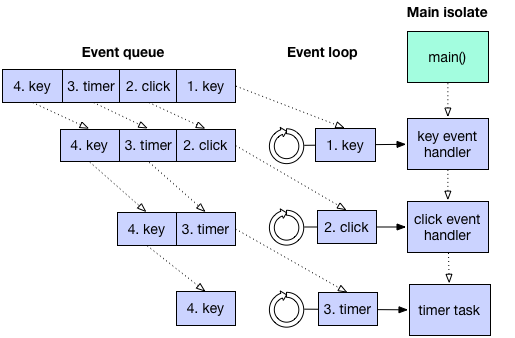
\includegraphics[scale=0.6]{dart.png}
	\caption{Funcionamiento del runtime de Dart}
	\end{figure}

\subsection{Diseño}
La parte de la solución que estamos implementando en este proyecto tiene unos inputs muy simples:
\begin{itemize}
	\item Activar alerta
	\item Desactivar alerta
	\item Escuchar alerta
	\item Cancelar escucha de alerta
\end{itemize}

\textbf{El FAB (floating action button)} que se situa abajo a la derecha realiza la primera, segunda y cuarta función. 
Cambia el icono central y su color dependiendo de la acción que dispara. En el caso de desactivar la alerta,
también se hace más grande para incluir un texto específico que podemos ver en la figura \ref{fig:alert}.

\begin{figure}[H]
	\centering	
	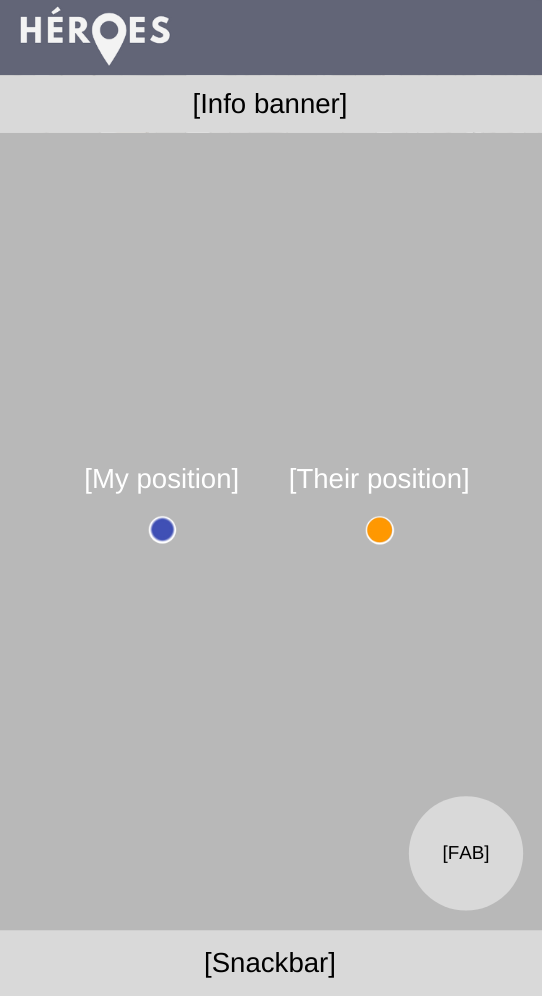
\includegraphics[scale=0.6]{mockup.png}
	\caption{Esquema de la aplicación}
	\end{figure}

Para escuchar una alerta, ha sido necesario incluir el \textbf{snackbar}, que emerge de la parte inferior de la aplicación cuando es necesario.
Esto es así, porque el usuario podría necesitar usar el FAB (en caso de necesitar ayuda) incluso si ha recibido una alerta. \\ \\

Por último, \textbf{para mostrar información tenemos el info banner y el mapa.} El primero informa al usuario una vez ha activado
una alerta de que esto se ha hecho con éxito, también informa de que se puede ver en el mapa la ubicación de la víctima en tiempo real
si está escuchando una alerta.

\subsection{Mapa}
En la aplicación, el mapa es muy protagonista. En él se ve representado el usuario y en caso de
atención a una alerta, también la víctima. \\ \\
Para implementarlo, \textbf{hay dos componentes:}
 \begin{itemize}
   \item \textbf{Provider de mapas:} Proporcionan los \textit{tiles}, que no son más que imágenes que forman el mapa. \textbf{OpenStreetMap, por ejemplo}. Se puede configurar por variables de entorno en la aplicación.
   \item \textbf{Controlador:} Su función es \textbf{cargar y mostrar los \textit{tiles} en la pantalla}, además de \textbf{reaccionar a los gestos que hace el usuario} para moverse por el mapa. 
 \end{itemize}

 Estoy utilizando OpenStreetMap como provider \cite{openstreetmap} por ser uno de los pocos que se pueden utilizar gratuitamente. \\ \\
 Como controlador, Map Controller Library \cite{map}, porque es bastante maduro, customizable y compatible con cualquier provider.

\begin{figure}[H]
	\centering	
	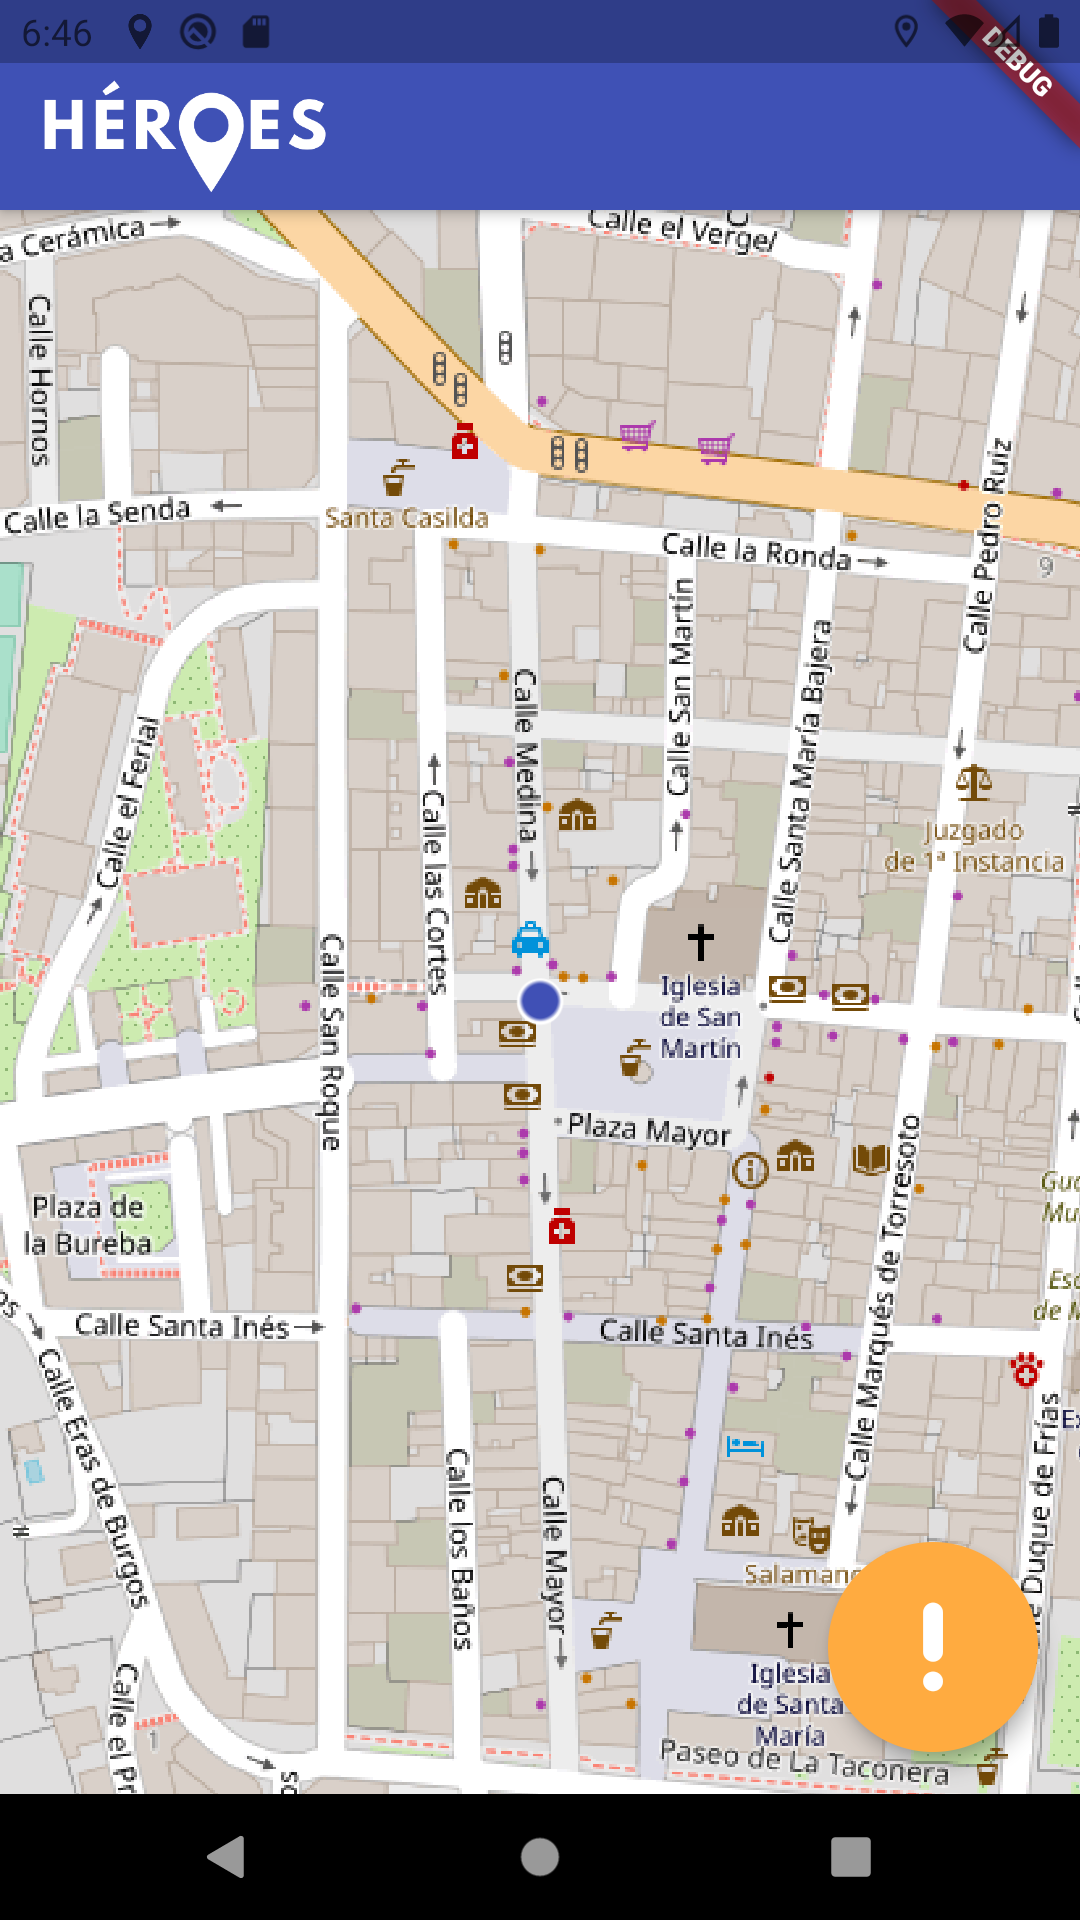
\includegraphics[scale=0.2]{home.png}
	\caption{Pantalla principal de la aplicación}
	\end{figure}

\subsection{Actualización de la localización}
Una parte fundamental de la aplicación es tener al día la ubicación del usuario para que \textbf{sea localizable en situación de alerta.} \\

En cualquiera de los siguientes escenarios:
\begin{itemize}
	\item La aplicación está en \textbf{primer plano.}
	\item La aplicación está \textbf{abierta en segundo plano.}
	\item La aplicación está \textbf{cerrada.}
\end{itemize}

Para ello, \textbf{he usado un isolate} (una hebra de Dart que se ejecuta aislada de la hebra principal, con un event loop independiente), que se comunica con la aplicación por medio de un Port (un canal entre hebras) y envía la ubicación actual al servidor. \\ \\
Además, usa APIs de Android que sacan partido a varios sensores del dispositivo para \textbf{disparar este 
proceso solo cuando el usuario realmente está en movimiento.}
También ha sido necesario registrar plugins como Firebase Cloud Messaging en java, para que estén disponibles en el isolate.

\subsection{Firebase Cloud Messaging}\label{sec:fib}
Como he anticipado en la sección \ref{sec:fibpre}, necesitamos un mecanismo para enviar notificaciones push a los usuarios en iOS y Android.
Además de integrar FCM en el servidor, también tenemos que hacerlo en el cliente para que las notificaciones lleguen en todos los escenarios.

\begin{itemize}
	\item La aplicación está en \textbf{primer plano.}
	\item La aplicación está \textbf{abierta en segundo plano.}
	\item La aplicación está \textbf{cerrada.}
\end{itemize}


Otra ventaja de usar FCM, es que nos permite obtener de manera sencilla un identificador único de dispositivo, que podemos usar en el servidor para enviar las notificaciones push.

\begin{figure}[H]
	\centering	
	
\includegraphics[scale=0.8]{notification.png}
	\caption{Notificación de alerta cuando la aplicación está cerrada}
	\end{figure}

\begin{figure}[H]
	\centering	
	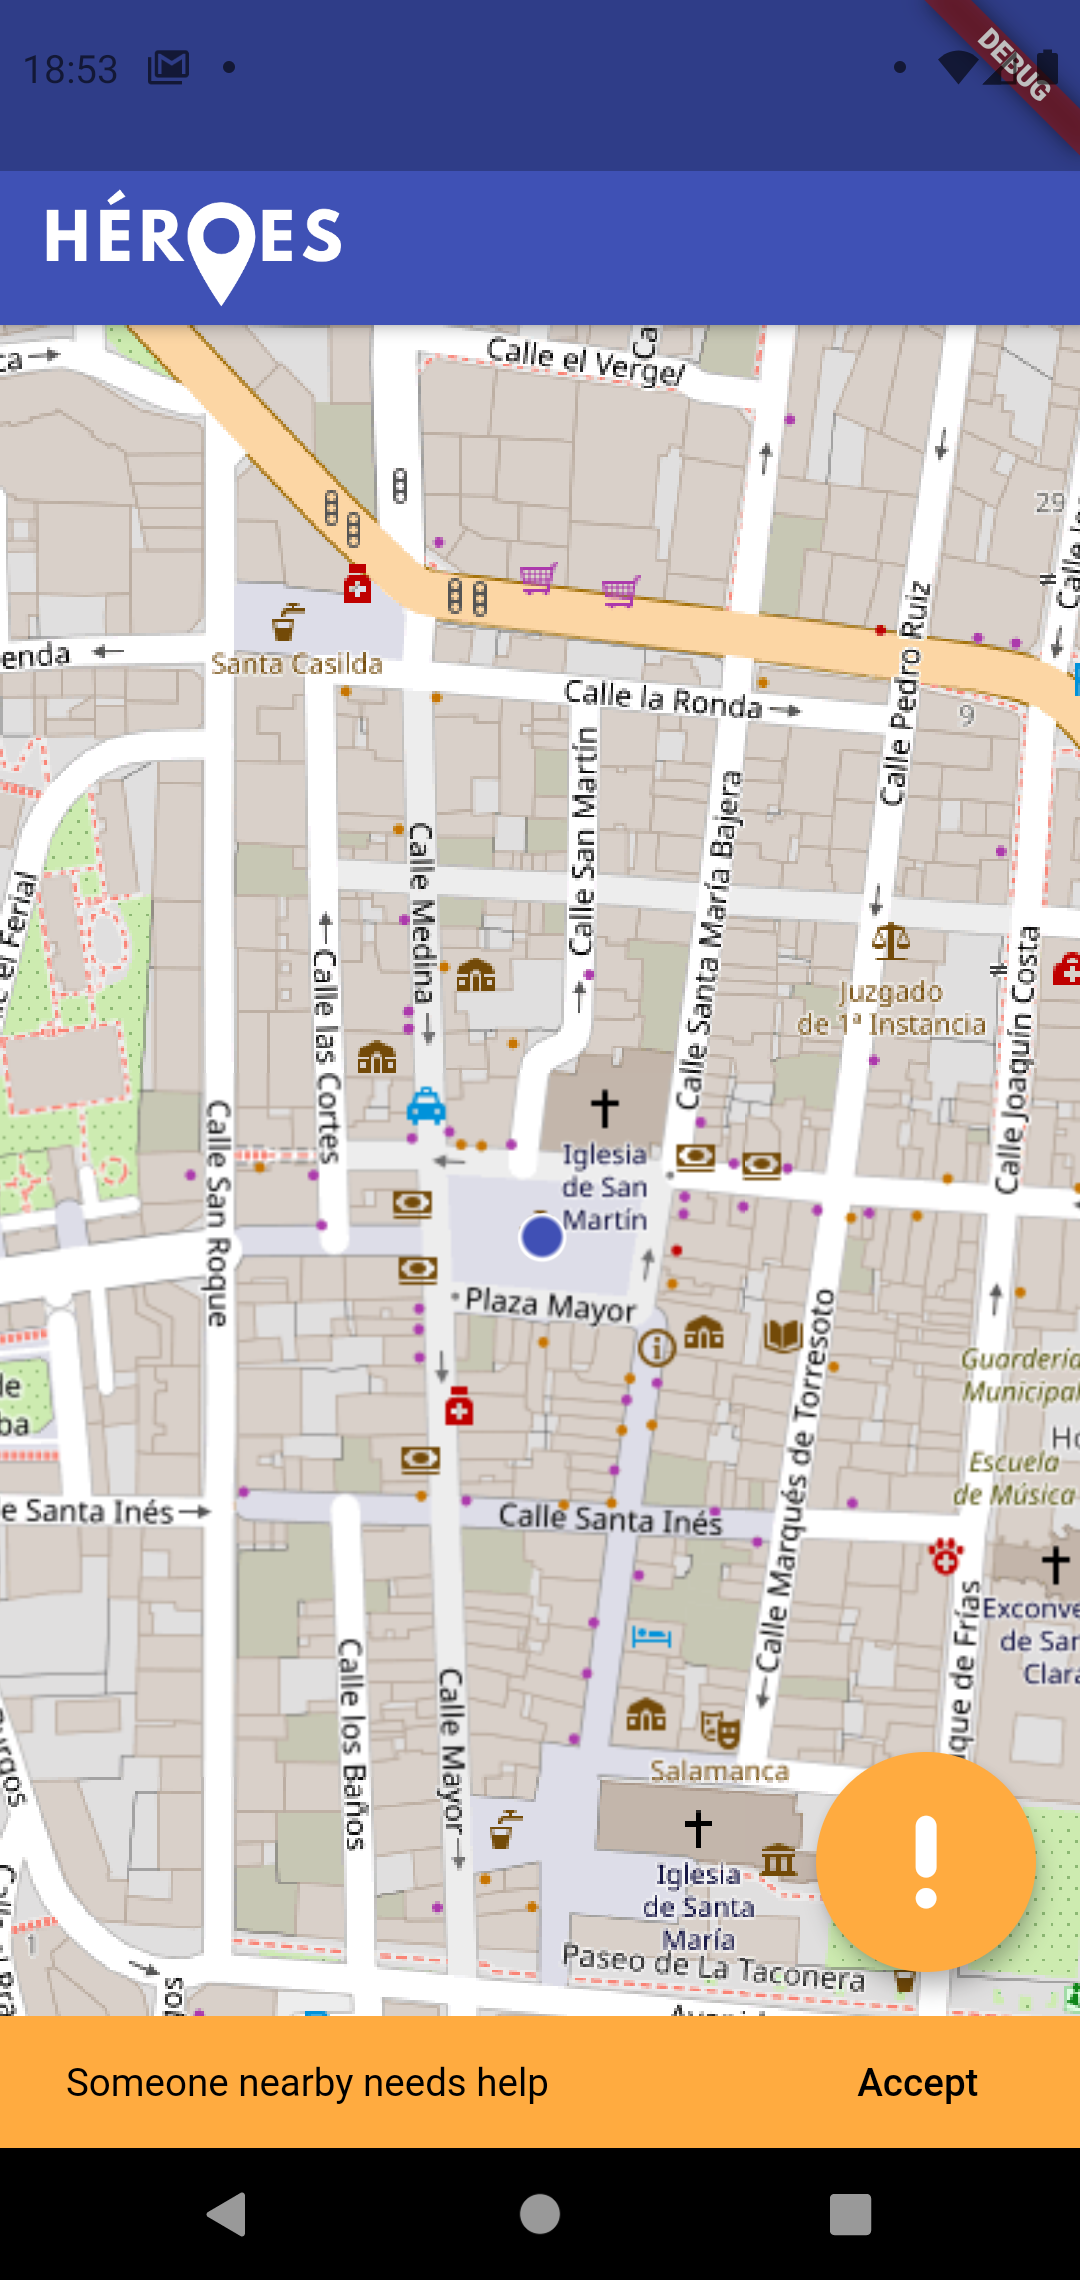
\includegraphics[scale=0.2]{notification-inapp.png}
	\caption{Notificación de alerta cuando la aplicación está abierta}
	\end{figure}

\subsection{Websockets}

Para obtener actualizaciones respecto a una alerta una vez la estamos escuchando, utilizamos el endpoint del que hemos hablado en \ref{subsec:websocket} mediante websockets.
He usado una librería \cite{websocketchannel} para esto.

\begin{figure}[H]
	\centering	
	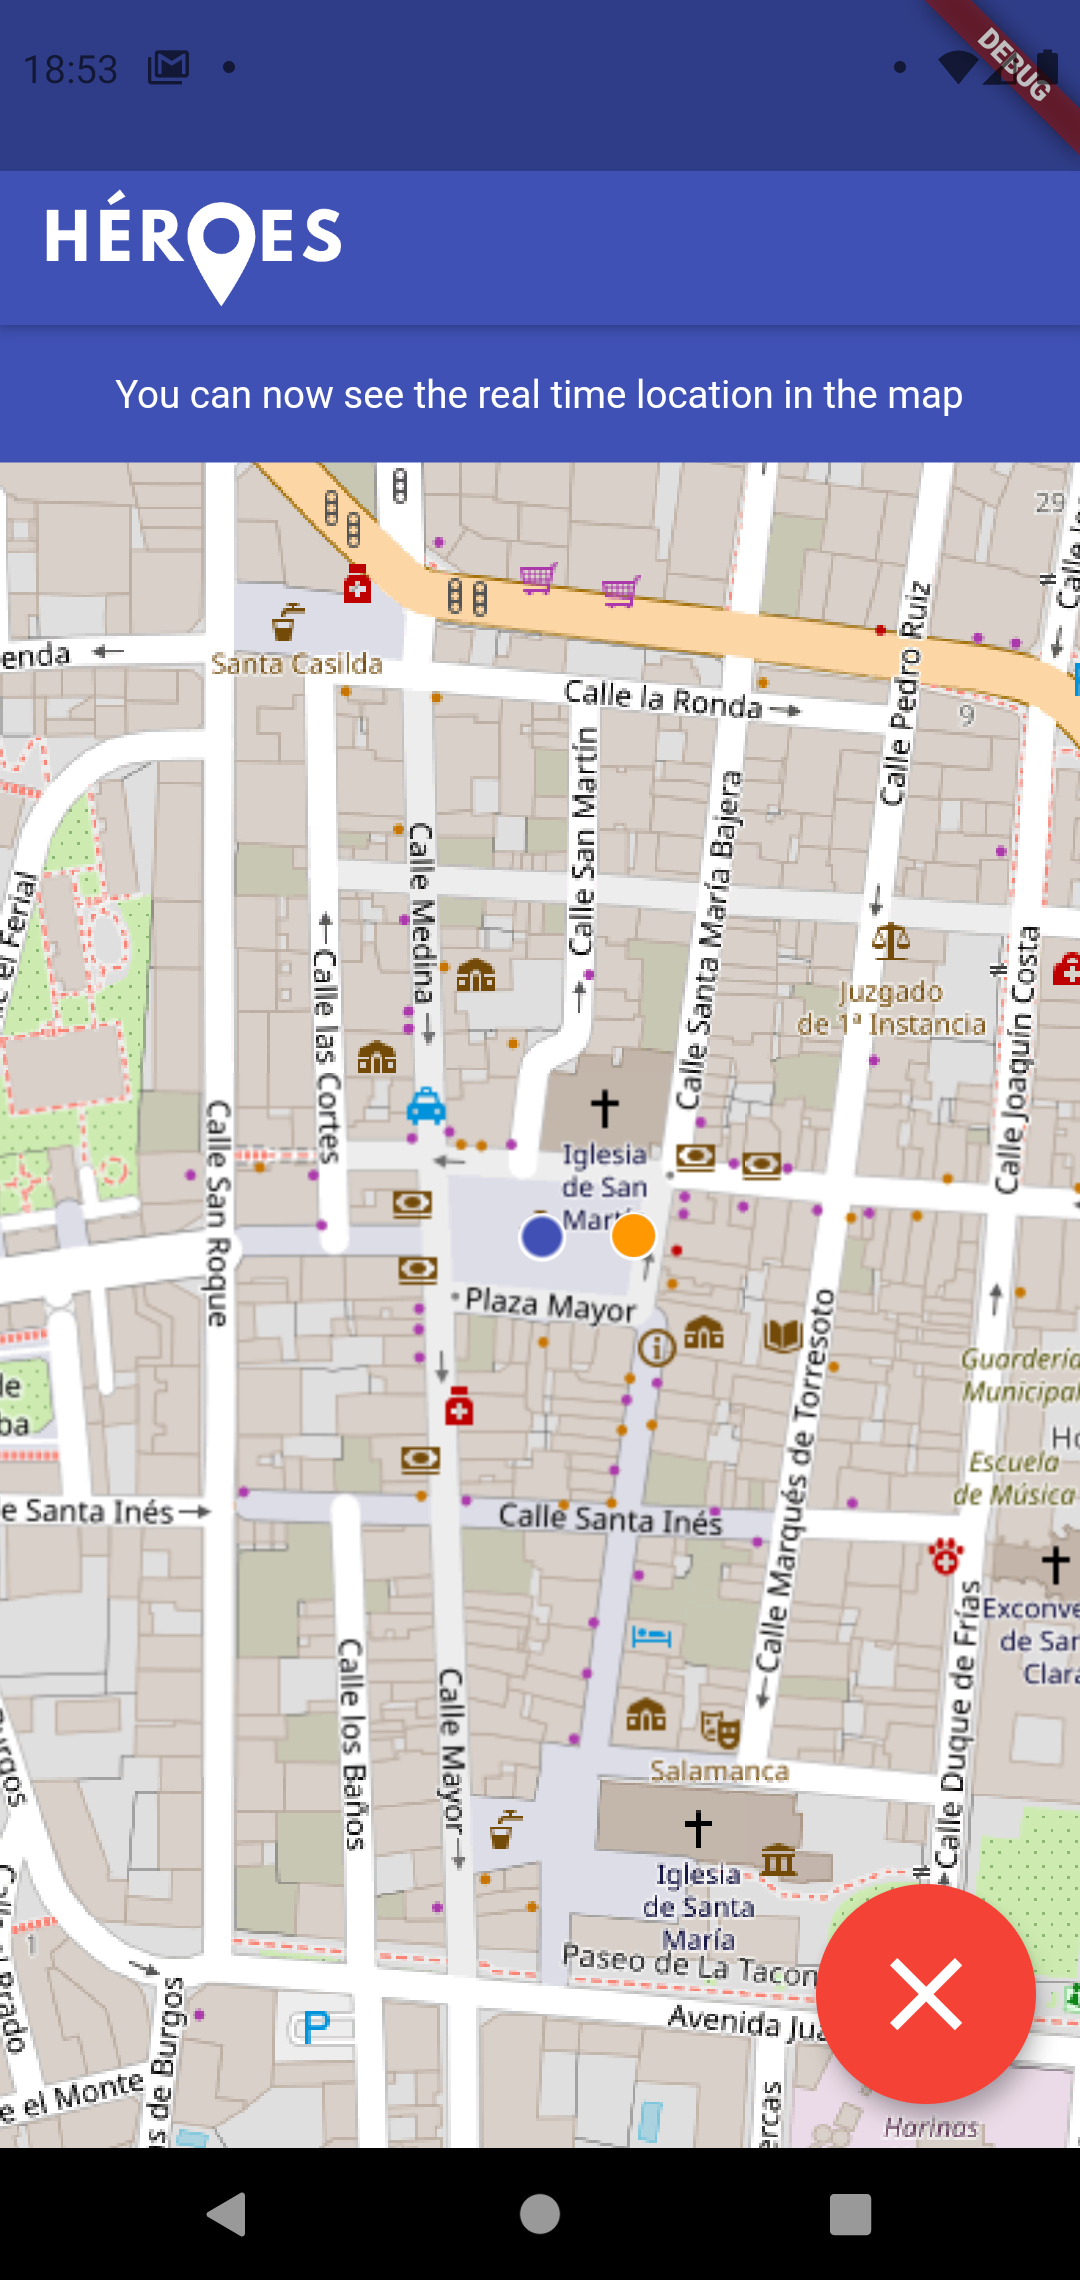
\includegraphics[scale=0.2]{watch-alert.png}
	\caption{Pantalla de seguimiento de alerta, actualización de la ubicación de la víctima y del estado de la alerta en tiempo real}
	\end{figure}

\subsection{Manejo del estado}
\textbf{En Flutter}, como en otros frameworks (React, Vue, Angular, etc...), \textbf{se crea un árbol de componentes.}
Los datos fluyen de arriba a abajo, de padres que saben más a hijos que saben
menos. Y los eventos de abajo a arriba, \textbf{los hijos informan a los padres de cambios mediante callbacks.}
\begin{figure}[H]
	\centering	
	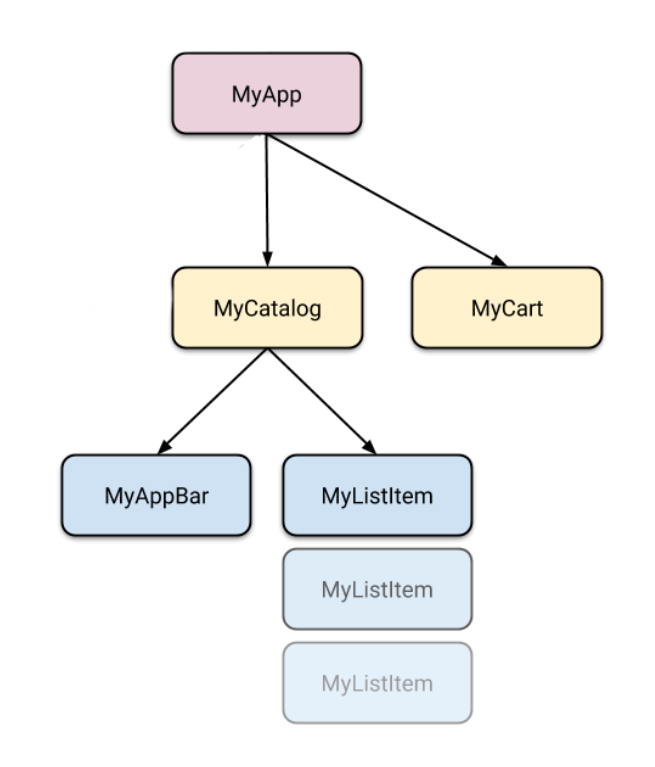
\includegraphics[scale=0.3]{tree.png}
	\caption{Un árbol de componentes. Fuente: Flutter docs \cite{state}}
	\end{figure}
Sin embargo, hay veces que \textbf{ciertos datos o comportamientos deben ser
expuestos para muchos componentes.} También puede pasar que no se necesiten
en componentes superficiales y sean necesarios en otros muy profundos. \\ \\
En un ecosistema tan grande como el de Flutter, tenemos varias propuestas, más y
menos sofisticadas. Redux, BLoC/Rx o MobX son algunos ejemplos, adecuadas
para casos más pesados.\\ \\
En mi opinión, \textbf{para aplicaciones pequeñas/medianas Provider es un \textit{sweet spot}
entre no usar estado de aplicación y usar uno muy potente.} \\ \\

Para esta aplicación, tiene mucho sentido, porque los datos no tienen estructura jerárquica, como, digamos, un e-commerce. \\
He utilizado dos providers que \textbf{exponen comportamiento y datos muy cohesionados:}
\begin{itemize}
	\item \textbf{Geolocalization provider:} Que ofrece getters y setters sobre el servicio de actualización en segundo plano y la localización actual.
	\item \textbf{Alert provider:} Que crea y realiza el seguimiento de alertas. También mantiene el estado sobre el rol del usuario (emitiendo alerta, standby, escuchando alerta, etc...).
\end{itemize}

\begin{figure}[H]\label{fig:alert}
	\centering	
	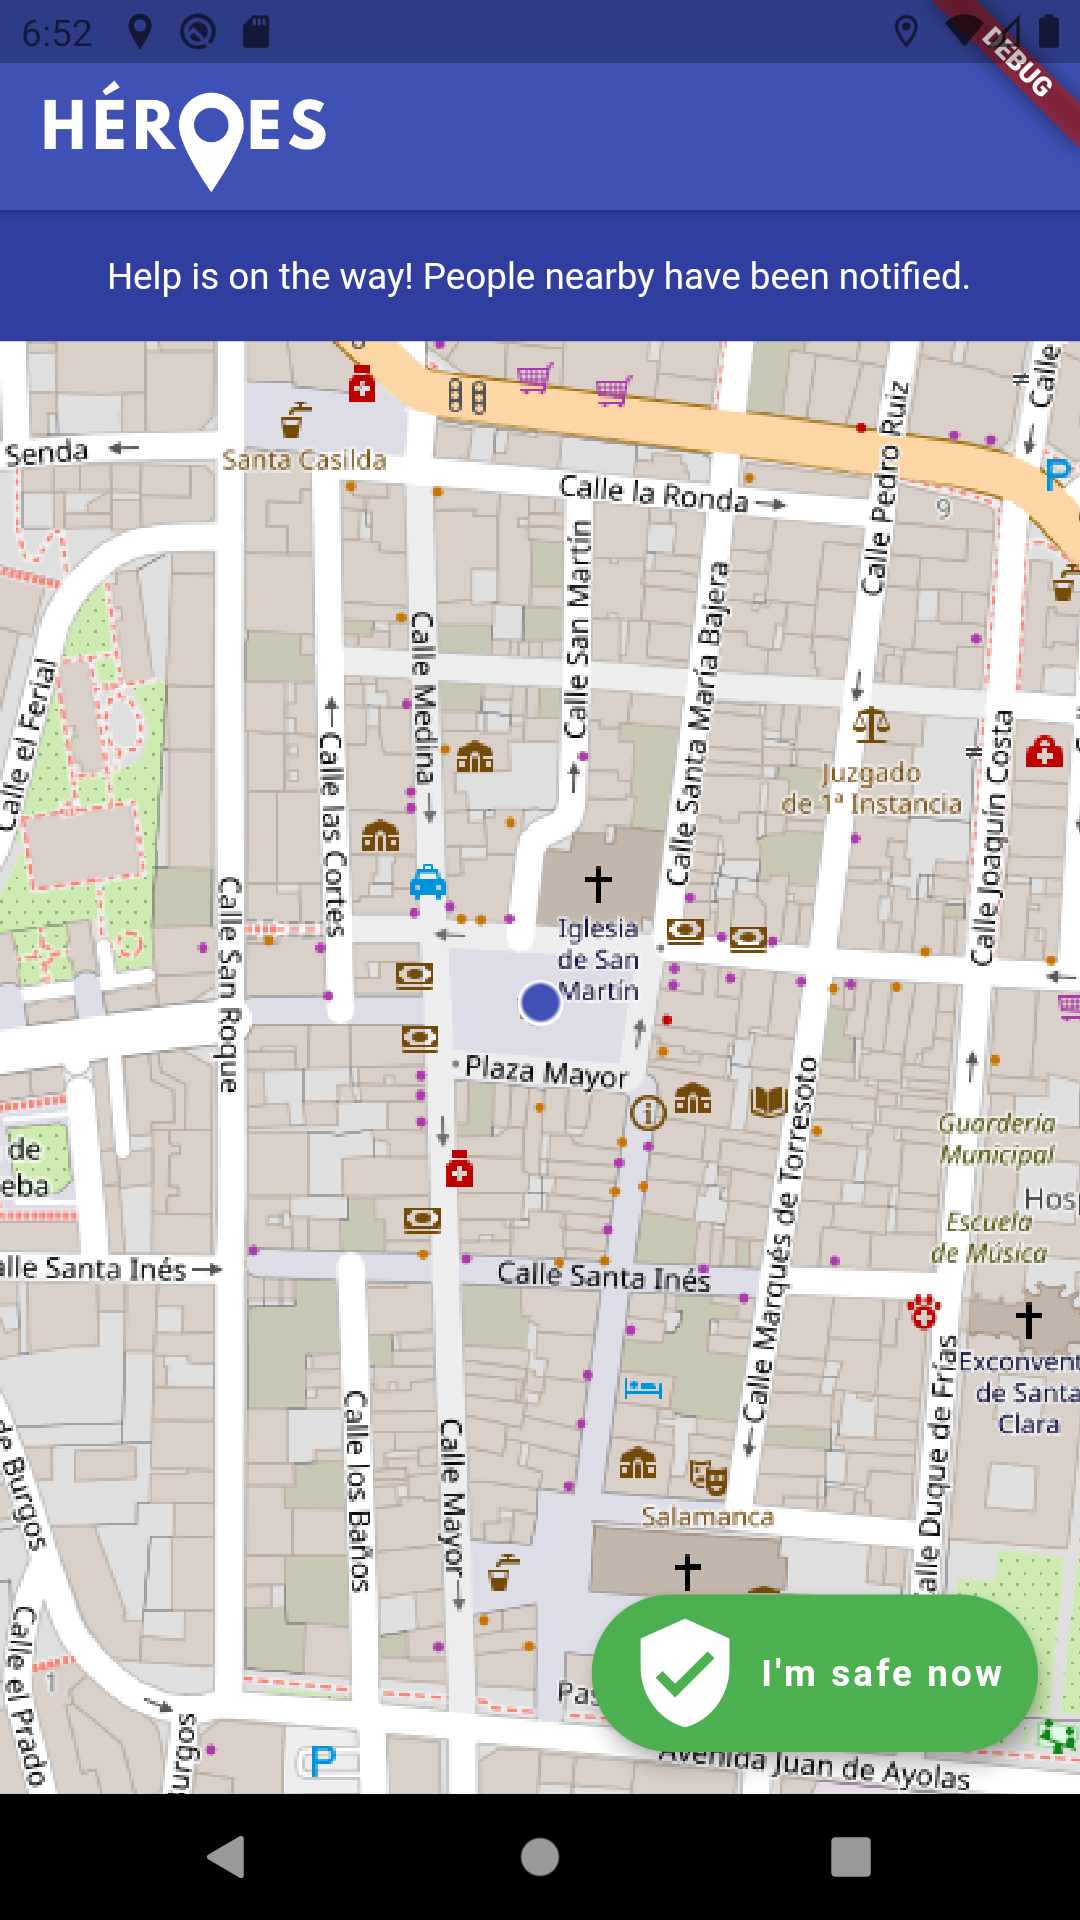
\includegraphics[scale=0.2]{create-alert.png}
	\caption{La aplicación después de crear una alerta. Los componentes reaccionan a cambios en los providers.}
	\end{figure}


	
	\newpage
	\bibliography{bibliografia}
	\bibliographystyle{plain}

	\appendix
	\chapter{Perfiles persona}

\section{Virginia}

\begin{itemize}
  \item \textbf{Nombre y apellidos: } Virginia Gómez
  \item \textbf{Nació en: } Villadiego
  \item \textbf{Reside en: } Burgos
  \item \textbf{Edad: } 18
  \item \textbf{Estado civil: } Soltera
  \item \textbf{Estudia: } Administración y dirección de empresas
  \item \textbf{Rasgos de personalidad: } 
  \begin{itemize}
    \item Divertida
    \item Carismática
    \item No muy independiente
    \item Deportista
  \end{itemize}
  \item \textbf{¿Cuáles son sus entornos?: } 
  \begin{itemize}
    \item Compañeros de clase y de la residencia de estudiantes.
    \item Amigos del pueblo.
    \item Su familia
  \end{itemize}
  \item \textbf{¿Qué influencia su opinión?: } 
  \begin{itemize}
    \item Lo que piensan sus amigos.
    \item Lo que lee en las redes sociales.
  \end{itemize}
  \item \textbf{Le gusta: } 
  \begin{itemize}
    \item Salir con sus amigas.
    \item Ver series.
    \item Ir al gimnasio.
    \item La música.
  \end{itemize}
  \item \textbf{No le gusta: } 
  \begin{itemize}
    \item Estudiar.
    \item Que le digan lo que tiene que hacer.
    \item Madrugar.
  \end{itemize}

\end{itemize}

\section{Carlos}

\begin{itemize}
  \item \textbf{Nombre y apellidos: } Carlos Martínez
  \item \textbf{Nació en: } Madrid
  \item \textbf{Reside en: } Madrid
  \item \textbf{Edad: } 27
  \item \textbf{Estado civil: } Soltero
  \item \textbf{Trabaja: } Profesor de educación física
  \item \textbf{Rasgos de personalidad: } 
  \begin{itemize}
    \item Serio.
    \item Cumplidor.
    \item Seguro de sí mismo.
    \item Deportista.
    \item Humilde.
  \end{itemize}
  \item \textbf{¿Cuáles son sus entornos?: } 
  \begin{itemize}
    \item Sus amigos del barrio.
    \item Compañeros de trabajo.
    \item Su familia y su pareja.
  \end{itemize}
  \item \textbf{¿Qué influencia su opinión?: } 
  \begin{itemize}
    \item Lo que ve en la tele.
    \item Lo que lee en las redes sociales.
    \item Lo que dice su pareja.
  \end{itemize}
  \item \textbf{Le gusta: } 
  \begin{itemize}
    \item Hacer escalada.
    \item Ver series.
    \item Ir al gimnasio.
    \item Ir a cenar con su pareja.
  \end{itemize}
  \item \textbf{No le gusta: } 
  \begin{itemize}
    \item La política.
    \item La chulería.
    \item El reggaeton.
    \item La navidad.
  \end{itemize}

\end{itemize}
	
\end{document}

